\setcounter{page}{2}

\section{Цель работы}

Целью лабораторной работы является ознакомление с существующими методиками предварительной оценки параметров программного проекта и практическая оценка затрат на примере методики COCOMO (COnstructive COst MOdel — конструктивная модель стоимости). 

\section{Модель оценки стоимости COCOMO}

Трудозатраты проекта --- количество человеко-месяцев --- в промежуточной модели COCOMO определяются по следующей формуле:

\begin{equation}
	\text{Трудозатраты } = C1 \cdot EAF \cdot (\text{Размер})^{P1}, \text{ где}
\end{equation}

\begin{itemize}
	\item $C1$ --- масштабирующий коэффициент;
	\item $EAF$ --- уточняющий фактор, характеризующий предметную область, персонал, среду и инструментарий, используемый для создания рабочих продуктов процесса, который является результатом учета 15 драйверов затрат;
	\item Размер --- размер конечного продукта (кода, созданного человеком), которые необходимы для реализации требуемой функциональной возможности (измеряется в тысячах строк кода $KLOC$);
	\item $P1$ --- показатель степени, характеризующий экономию при больших масштабах, присущую тому процессу, который используется для создания конечного продукта; в частности, способность процесса избегать непроизводительных видов деятельности (доработок, бюрократических проволочек, накладных расходов на взаимодействие).
\end{itemize}

Время проекта --- общее количество месяцев --- определяется по следующей формуле:

\begin{equation}
	\text{Время } = C2 \cdot(\text{Трудозатраты})^{P2}, \text{ где}
\end{equation}

\begin{itemize}
	\item $C2$ --- масштабирующий коэффициент для сроков исполнения;
	\item $P2$ --- показатель степени, который характеризует инерцию и распараллеливание, присущие управлению разработкой программного обеспечения.
\end{itemize}

При этом могут поддерживаться разные режимы проекта, драйверы затрат выбираются в соответствии с характеристиками разрабатываемого проекта.

На рисунке~\ref{fig:screen1} приведеыны значения драйверов затрат в модели COCOMO.

\begin{figure}[H]
	\centering
	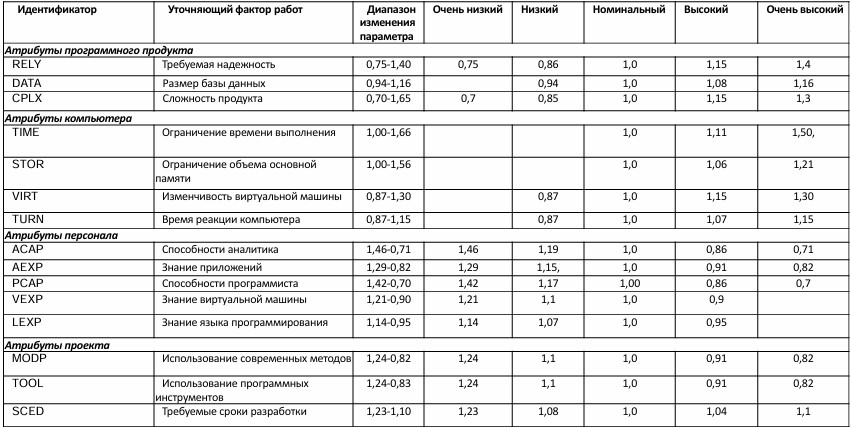
\includegraphics[width=0.9\textwidth]{img/screen1.jpg}
	\caption{Значение драйверов затрат в модели COCOMO}
	\label{fig:screen1}
\end{figure}

\section{Задание 1}

\subsection{Условие задания}

Исследовать степень влияния различных драйверов затрат на трудоемкость (РМ) и время разработки (ТМ) для промежуточной модели COCOMO. Для этого проанализировать, как меняется трудоемкость и время выполнения проекта при различных уровнях автоматизации среды:

\begin{itemize}
	\item драйвер MODP --- использование современных методов;
	\item драйвер TOOL --- использование программных инструментов;
\end{itemize}

и разном уровне способностей ключевых членов команды:

\begin{itemize}
	\item драйвер ACAP --- способности аналитика;
	\item драйвер PCAP --- способности программиста.
\end{itemize}

Взять за основу промежуточный тип проекта и при фиксированном значении размера программного кода (SIZE) получить значения PM и ТМ, изменяя значения указанных драйверов от очень низких до очень высоких. Результаты исследований оформить графически и сделать соответствующие выводы. 

При необходимости сократить срок выполнения проекта, что повлияет больше: способности персонала или параметры среды? 

При высоком уровне автоматизации (оба драйвера MODP и TOOL высокие) что окажет большее влияние на трудоемкость и время выполнения:  высокая надежность (параметр RELY повышается 
от номинального до высокого) или требование заказчика, чтобы не менее 70\% компонентов разрабатываемого ПО могло использоваться в режиме реального времени (драйвер TIME повышается от 
номинального до высокого)?

\subsection{Выполнение задания}

На рисунке~\ref{fig:screen2} приведена зависимость трудозатрат и времени разработки от уровня способностей персонала (драйверы ACAP и PCAP) и уровня автоматизации среды (драйверы MODP и TOOL).

\begin{figure}[H]
	\centering
	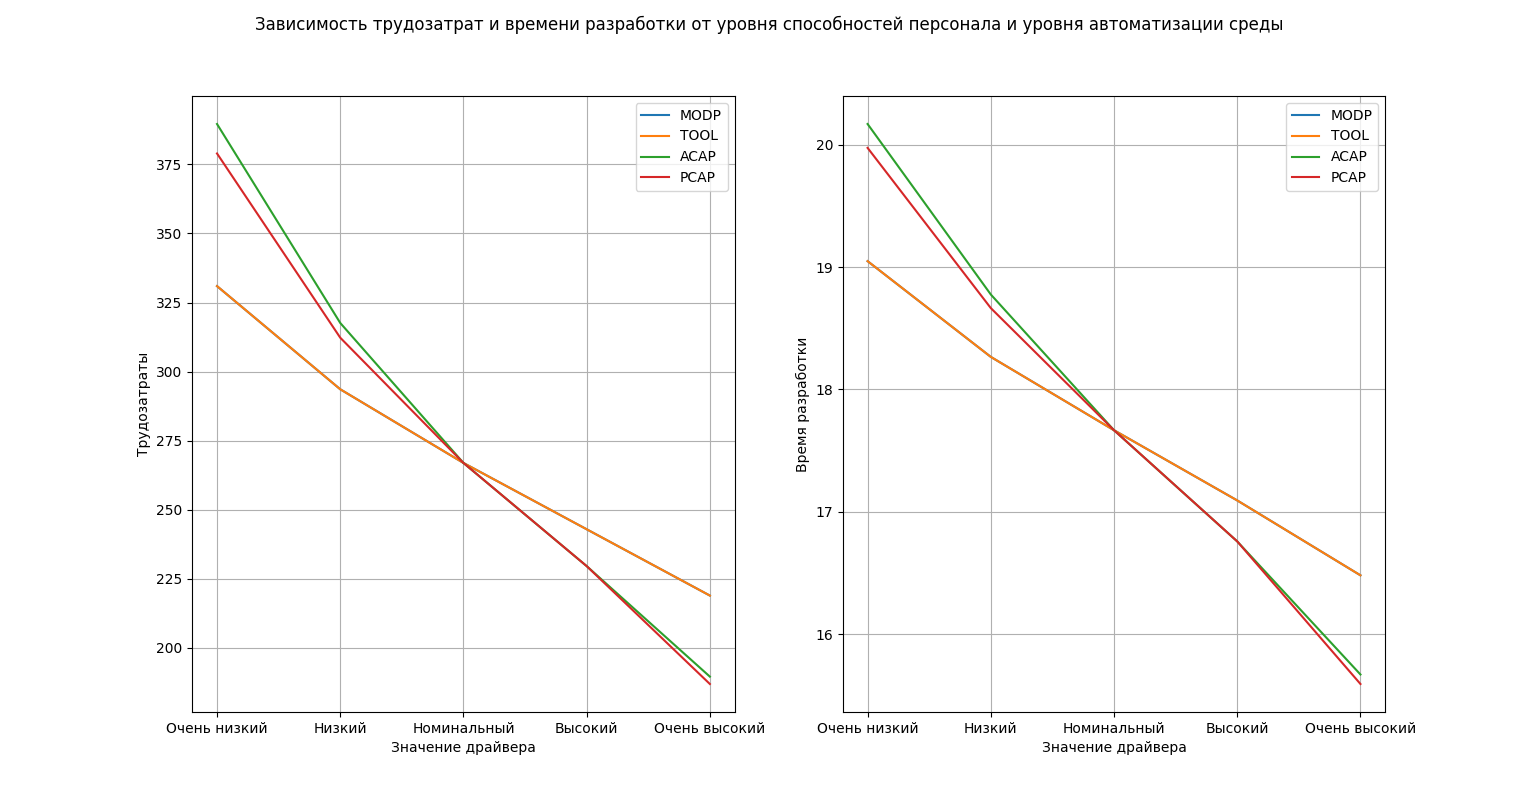
\includegraphics[width=0.9\textwidth]{img/task1_1.png}
	\caption{Зависимость трудозатрат и времени разработки от уровня способностей персонала и уровня автоматизации среды}
	\label{fig:screen2}
\end{figure}

При увеличении уровня использования современных методов MODP, использования программных инструментов TOOL, способностей аналитика ACAP и способностей программистов PCAP трудозатраты и время разработки уменьшаются, причем влияние MODP и TOOL совпадает, а ACAP и PCAP (уровень способностей команды) вносят больший вклад в снижение временных и трудозатрат.
Тем самым при необходимости сократить срок выполнения проекта больше повлияют способности персонала.
При этом больший вклад вносят способности аналитика.

На рисунке~\ref{fig:screen3} приведена зависимость трудозатрат и времени от надежности и ограничений времени выполнения при высоких MODP и TOOL.

\begin{figure}[H]
	\centering
	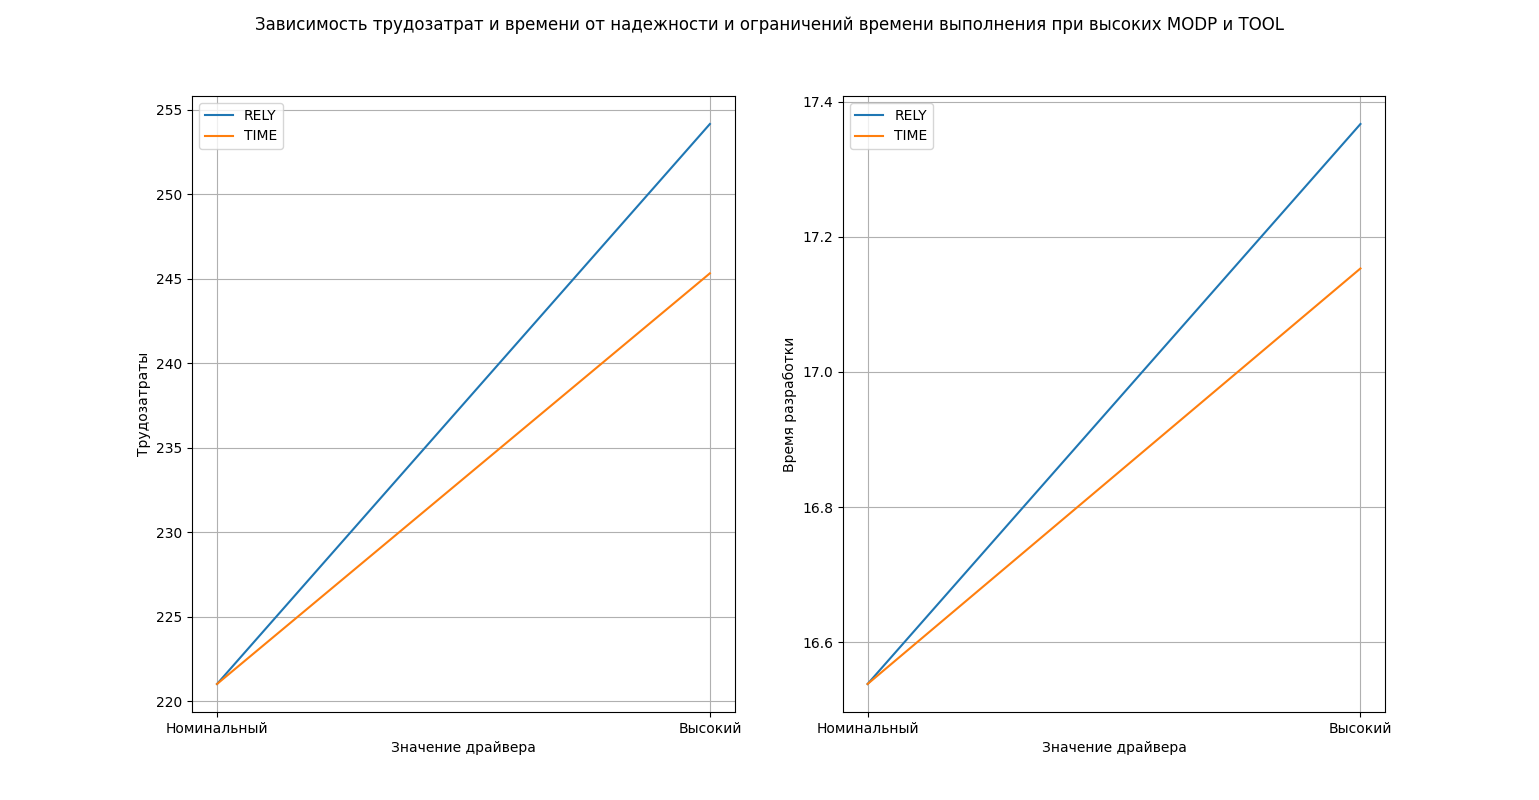
\includegraphics[width=0.9\textwidth]{img/task1_2.png}
	\caption{Зависимость трудозатрат и времени от надежности и ограничений времени выполнения при высоких MODP и TOOL}
	\label{fig:screen3}
\end{figure}

При высоком уровне автоматизации большее влияние на рост трудозатрат и времени выполнения оказывает требование к высокой надежности.

\section{Задание 2}

\subsection{Условие задания}

При разработке программного продукта его размер оценивается примерно в 55 KLOC. Этот проект будет представлять собой Web систему, снабженную устойчивой серверной базой данных. 
Предполагается применение промежуточного варианта. Проект предполагает создание продукта средней сложности с номинальными требованиями по надежности, но с расширенной базой данных. 
Квалификация персонала средняя, однако способности аналитика высокие. Оценить параметры проекта.

\subsection{Выполнение задания} 

Из условия:

\begin{itemize}
	\item режим проекта --- промежуточный;
	\item $KLOC = 55$;
	\item размер базы данных DATA --- высокий;
	\item способности аналитика ACAP --- высокие;
	\item прочие драйверы затрат --- номинальные.
\end{itemize}

Тогда:

\begin{itemize}
	\item $C1 = 3, P1 = 1.12$;
	\item $EAF = 1^{13} \cdot 1.08 \cdot 0.86 = 0.9288$;
	\item $\text{Трудозатраты } = 3 \cdot 0.9288 \cdot 55^{1.12} = 247.88 \text{ человеко-месяца}$ (без планирования и определения требований);
	\item $C2 = 2.5, P2 = 0.35$;
	\item $\text{Время } = 2.5 \cdot 247.88^{0.35} = 17.22 \text{ месяцев}$  (без планирования и определения требований).
\end{itemize}

На рисунке \ref{fig:screen4} приведены распределение работ и времени по стадиям жизненного цикла и распределение работ по видам деятельности WBS.

\begin{figure}[H]
	\centering
	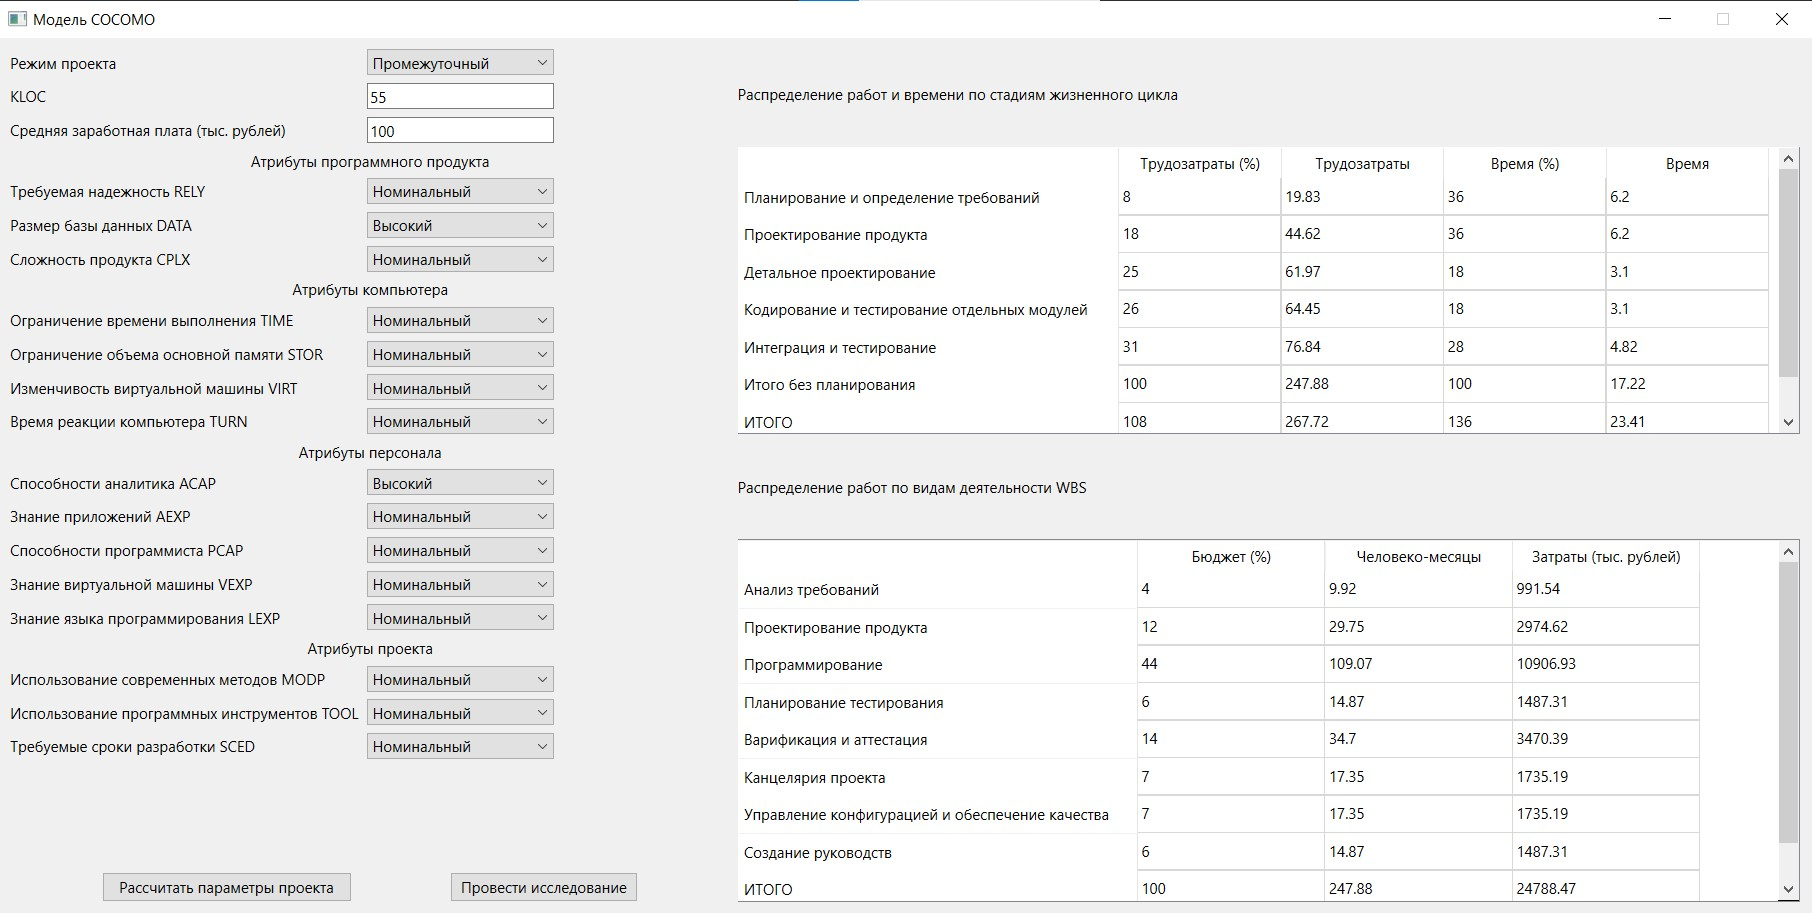
\includegraphics[width=0.9\textwidth]{img/task2_1.jpg}
	\caption{Оценка параметров проекта с использованием COCOMO}
	\label{fig:screen4}
\end{figure}

Наибольшие затраты приходятся на программирование (10906 тыс. рублей).

Требуемое для этапа выполнения проекта число сотрудников вычисляется следующим образом:

\begin{equation}
	\text{Число сотрудников} = \frac{\text{Трудозатраты}}{\text{Время}}.
\end{equation}

На рисунке \ref{fig:screen5} показана диаграмма привлечения сотрудников, где

\begin{itemize}
	\item 1 --- планирование и определение требований;
	\item 2 --- проектирование продукта;
	\item 3 --- детальное проектирование;
	\item 4 --- кодирование и тестирование отдельных модулей;
	\item 5 --- интеграция и тестирование.
\end{itemize}

\begin{figure}[H]
	\centering
	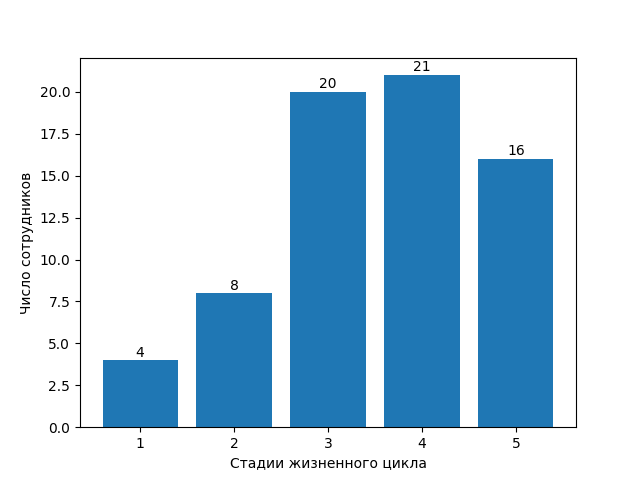
\includegraphics[width=0.9\textwidth]{img/task2_2.png}
	\caption{Диаграмма привлечения сотрудников}
	\label{fig:screen5}
\end{figure}

Наибольшее число сотрудников понадобится на этап кодирования и тестирования (21 человек).

Предварительную оценку бюджета проекта можно определить так:

\begin{equation}
	\text{Бюджет} = \text{Трудозатраты}\cdot\text{Средняя заработная плата}.
\end{equation}

Для средней заработной платы 100~000 рублей проект обойдется в 24~788~470 рублей.

\section*{Вывод}

Использование модели COCOMO позволяет выполнить предварительную оценку трудозатрат, времени выполнения и стоимости проекта, варьируя параметры проекта.

С использованием модели COCOMO можно выполнить предварительную оценку трудозатрат, длительности выполнения и стоимости проекта. При этом методика позволяет производить расчеты для проектов разных масштабов с учетом их индивидуальных характеристик и проста в применении. Но у модели есть недостатки, влияющие на точность оценок:

\begin{itemize}
	\item расчеты в модели зависят от размера проекта, поэтому точность оценки проекта зависит от точности оценки размера;
	\item методика основана на каскадной модели жизненного цикла, поэтому не учитывает тонкости других методологий;
	\item поверхностное внимание к вопросам безопасности и надежности;
	\item не учитывается повторное использование компонентов, что влияет на размер проекта.
\end{itemize}
